\section{Problem Setup and Methods}
\label{sec:method}

\subsection{Safety Commitment Point}
\label{sec:commitment-point}

When a reasoning model is jailbroken, its chain-of-thought (CoT) transitions from safety-aware deliberation to committed harmful generation. We define the \textbf{Safety Commitment Point} (CP) as the first reasoning step after which safety deliberation permanently ceases; traces with oscillating safety deliberation are resolved by taking the final irreversible transition. This binary formulation is a deliberate simplification; we discuss its limits in \cref{sec:limitations}. Steps before CP are \emph{pre-commitment} ($y_t = 0$); steps at or after CP are \emph{post-commitment} ($y_t = 1$). The classification task produces a score $s_t \in [0, 1]$ estimating whether the model has passed its CP by step $t$. Annotation quality is robust to boundary uncertainty: shifting CP labels by $\pm$1 step changes balanced accuracy by ${<}2.5$pp (\cref{tab:cp_perturbation}).

We study four reasoning models spanning two architectures and two scales (\cref{tab:models}).

\begin{table}[t]
\centering
\resizebox{\columnwidth}{!}{%
\begin{tabular}{lccccc}
\toprule
\textbf{Model} & \textbf{Arch.} & \textbf{Params} & \textbf{Layers} & \textbf{Hidden} & \textbf{$n$ (total\,/\,test)} \\
\midrule
R1-8B & Llama & 8B & 32 & 4096 & 209\,/\,43 \\
OT-7B & Qwen & 7B & 28 & 3584 & 228\,/\,47 \\
R1-32B & Qwen & 32B & 64 & 5120 & 100\,/\,20 \\
QwQ-32B & Qwen & 32B & 64 & 5120 & 95\,/\,19 \\
\bottomrule
\end{tabular}}
\caption{Models studied. R1-8B and R1-32B are distilled from DeepSeek-R1~\citep{deepseekr1}; QwQ-32B~\citep{qwq} is a native reasoning model; OT-7B~\citep{openthinker} is trained with STILL~\citep{still} on Qwen2.5-7B. Data: HarmThoughts~\citep{harmthoughts} with step-level CP annotations (CP = first reasoning step after which safety deliberation permanently ceases). Split: 60/20/20.}
\label{tab:models}
\end{table}

\subsection{Probe Architecture}
\label{sec:probe-architecture}

\paragraph{Hidden-state (HS) probes.} At each step $t$, we extract the last-token hidden state $\mathbf{h}_t^{(\ell)} \in \mathbb{R}^d$ from layer $\ell$ and train an L2-regularized logistic regression classifier (balanced class weights, $C{=}1.0$, LBFGS, max\_iter${}=2000$) on binary CP labels. Sweeping $C \in [0.01, 100]$ yields $<$2pp BA variation (\cref{app:hyperparameter_robustness}), confirming robustness to this default. Layer selection is analyzed in \cref{sec:layer-sensitivity}.

\paragraph{Text probes.} Each step's text is encoded with all-MiniLM-L6-v2~\citep{wang2020minilm} ($\mathbb{R}^{384}$), a distilled sentence encoder from the Sentence-BERT family~\citep{reimers2019sentence}. The same logistic regression is applied as a surface-level modality baseline.

\paragraph{Temporal windowing.} For window size $W$, we concatenate features from steps $[t{-}W{+}1, \ldots, t]$. We evaluate $W \in \{1, 3, 5, 10, 15, 20, 25\}$ and select per-model on validation. GRU sequence models are also evaluated under two protocols: a 70/30 train/test split (primary) and the same 60/20/20 split used for LR experiments (for fair comparison; \cref{tab:gru_multi_seeds,app:gru_details}).

\subsection{Layer Selection Sensitivity}
\label{sec:layer-sensitivity}

Layer selection is a researcher degree of freedom that can reverse modality comparison conclusions. We evaluate five metrics: balanced accuracy (BA), precision, and inverse false positive rate (FPR) are standard probing metrics~\citep{belinkov2022probing}; crossing rate measures the fraction of traces where the probe score exceeds a threshold for $K$ consecutive steps~\citep{kaya2019shallow,zhou2020bert}; and additive composite combines precision with inverse FPR. A multiplicative composite (BA $\times$ crossing rate) serves as the \emph{crossing-rate composite} (CR-composite). Metrics at a fixed decision threshold (precision, inverse FPR, additive composite) form the \emph{threshold-based} selection. Crossing rate inflates at shallow layers where representations are compressed: inter-step cosine distances are 1.4--2.7$\times$ smaller (\cref{fig:cosine_compression,app:cosine_volatility}), causing a linear probe to operate near the noise floor. Threshold-based metrics converge to deep layers; BA independently confirms. This predicts a priori that CR-composite exhibits shallow-layer bias, confirmed by results (\cref{sec:layer-results}); full per-layer sweeps in \cref{app:layer_sweep}.\looseness=-1

\begin{figure}[t]
\centering
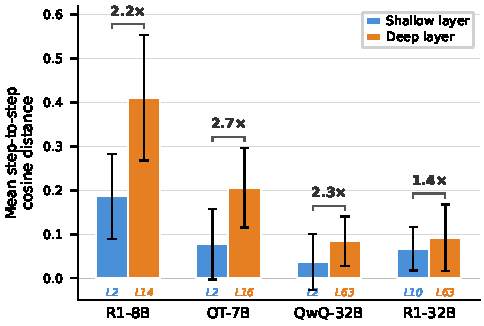
\includegraphics[width=\columnwidth]{figures/fig_cosine_compression.pdf}
\caption{Cosine compression at shallow vs.\ deep layers. Shallow layers produce compressed representations (1.4--2.7$\times$ smaller inter-step cosine distances), causing spurious threshold crossings that inflate crossing rate. Layer indices below each bar; compression ratios above. Error bars: $\pm$1 std. Data from \cref{tab:cosine_volatility}.}
\label{fig:cosine_compression}
\end{figure}

\subsection{Baseline Methods}
\label{sec:baselines}

We evaluate seven alternatives to contextualize probe performance (\cref{tab:negative}): Bayesian online change-point detection (BOCPD)~\citep{adams2007bayesian} and cumulative sum (CUSUM)~\citep{page1954cusum} for change-point detection; Mahalanobis distance following TrajGuard~\citep{trajguard}; RepE mean-difference directions~\citep{zou2023representation}; two-layer MLP probes; CCS-adapted~\citep{burns2023discovering}; and cross-model transfer via PCA. A position-only baseline ($t/T$) controls for temporal artifacts. Detailed configurations in \cref{app:bocpd_config,app:transfer_details}.

\subsection{Evaluation Protocol}
\label{sec:evaluation}

We report balanced accuracy, precision, pre-CP FPR, coverage, and lead time. We exclude F1 (conflates precision and recall), area under the ROC curve (AUROC; threshold-free, cannot diagnose layer selection bias), and Matthews correlation coefficient (MCC; redundant with BA under balanced priors). Positive classification requires $K{=}5$ consecutive threshold crossings, selected on the R1-8B validation set and held fixed across all models as the value balancing coverage ($\geq$70\%) and safe-trace false positive rate ($\leq$50\%); per-model optimal $K$ values range from 3 to 7 (\cref{tab:k_ablation}), and the HS vs.\ text conclusion direction is consistent at $K{=}3$, $5$, and $7$ (\cref{app:threshold_sensitivity}), with coverage and FPR trading off monotonically. Modality comparisons use bias-corrected and accelerated (BCa) bootstrap (10{,}000 resamples, resampling traces as clusters: each trace is an independent unit and all its steps are included or excluded together, preserving within-trace dependence)~\citep{efron1993bootstrap,diciccio1996bootstrap} with Holm-Bonferroni (HB) step-down (3 metrics $\times$ 4 models $= 12$ tests, $\alpha{=}0.05$); the 4-test framework yields identical conclusions (\cref{app:holm_bonferroni}). For 32B models ($n \leq 20$), the exact permutation test is the primary inference method; BCa confidence intervals are reported for comparability but may have reduced coverage at these sample sizes (BCa assumes approximate pivotality; heavy-tailed score distributions could produce anti-conservative intervals). Within each model, the three metrics are positively correlated, so the correction is stricter than under independence. Control task selectivity~\citep{hewitt2019control} validates genuine structure (\cref{app:control}). $\dagger$ marks sample-limited test sets ($n \leq 20$): R1-32B ($n{=}20$) and QwQ-32B ($n{=}19$).

\paragraph{Multiple comparisons.} The full search spans ${\sim}$980--2{,}240 configurations per model; the effective number of independent tests is far smaller (shared confusion matrix, adjacent-layer correlation; \cref{app:effective_tests}). A two-stage design protects against selection bias: upstream exploration uses nested CV at 7--8B; downstream tests apply HB to 12 comparisons. 32B models lack nested cross-validation (CV) and are marked exploratory ($\dagger$). Details in \cref{app:effective_tests}.\looseness=-1

